
\de{ĐỀ THI HỌC KỲ I NĂM HỌC 2022-2023}{THPT Tạ Quang Bữu}


\begin{bt}%[0T3Y1-2]%[Dự án đề kiểm tra HKI NH22-23- Phan Trung Hiếu]%[THPT Tạ Quang Bửu]
	 Tìm tập xác định của các hàm số sau
	\begin{enumerate}
		\item $y=\sqrt{5-2 x}$.
		\item  $y=\dfrac{1}{2 x+6}$.
	\end{enumerate}
	\dapso{ a) $\left(-\infty;\dfrac{5}{2}\right]$ ; b) $\mathbb{R}\setminus \{-3\}$ }
	\loigiai{
		\begin{enumerate}
			\item Điều kiện $5-2x\geq 0\Leftrightarrow x\leq\dfrac{5}{2}$.\\
			Vậy tập xác định của hàm số là $\mathscr{D}=\left(-\infty;\dfrac{5}{2}\right]$.
			\item Điều kiện $2x+6\ne0\Leftrightarrow x\ne-3$.\\
			Vậy tập xác định của hàm số là $\mathscr{D}=\mathbb{R}\setminus\{-3\}$.
		\end{enumerate}
	}
\end{bt}
\begin{bt}%[0T3T1-2]%[Dự án đề kiểm tra HKI NH22-23- Phan Trung Hiếu]%[THPT Tạ Quang Bửu]
	Dự báo thời tiết ngày $01 / 5 / 2021$ tại Thành phố Hồ Chí Minh được cho trong bảng sau
	\begin{center}
		\begin{tabular}{|c|c|c|c|c|c|c|c|c|}
			\hline Giờ & 1 & 4 & 7 & 10 & 13 & 16 & 19 & 22 \\
			\hline Nhiệt độ $\left({ }^{\circ} \mathrm{C}\right)$ & 28 & 27 & 28 & 32 & 31 & 29 & 28 & 27 \\
			\hline
		\end{tabular}
	\end{center}
	
Biết rằng bảng dữ liệu dự báo thời tiết là một hàm số, hãy tìm tập xác định của hàm số đó?
	\dapso{$\{1;4;7;10;13;16;19;22\}$  }
	\loigiai{
		Tập xác định của hàm số là $\mathscr{D}=\{1;4;7;10;13;16;19;22\}$.
	}
\end{bt} 
\begin{bt}%[0T1B3-1]%[Dự án đề kiểm tra HKI NH22-23- Phan Trung Hiếu]%[THPT Tạ Quang Bửu]
	\begin{enumerate}
		\item Cho các tập hợp  $A=\{0 ; 2 ; 4 ; 6 ; 8\}$, $B=\{0 ; 3 ; 6 ; 9\}$. Xác định các tập hợp $A \setminus B$, $B \cap A$.
		\item Cho các tập $C=[-2 ; 1)$, $D=(0 ; 3]$. Xác định các tập hợp $C \cap D$, $D\setminus C$.
	\end{enumerate}
	\dapso{ a) $A\setminus B=\{2;4;8\}$; $B\cap A=\{0;6\}$ ; b) $C\cap D=(0;1)$; $D\setminus C=\left[1;3\right]$ }
	\loigiai{
		\begin{enumerate}
			\item $A\setminus B=\{2;4;8\}$; $B\cap A=\{0;6\}$.
			\item $C\cap D=(0;1)$; $D\setminus C=\left[1;3\right]$.
		\end{enumerate}
	}
\end{bt}
\begin{bt}%[0T2K2-3]%[Dự án đề kiểm tra HKI NH22-23- Phan Trung Hiếu]%[THPT Tạ Quang Bửu]
	Biểu diễn miền nghiệm của hệ bất phương trình $\heva{&3 x+y \leq 5 \\& x+2 y \leq 4 \\& x \geq 0 \\ &y \geq 0.}$ \\
	\dapso{Miền nghiệm là miền tứ giác $OABC$ với $O(0;0)$, $A(0;2)$, $B\left(\dfrac{6}{5};\dfrac{7}{5}\right)$, $C\left(\dfrac{5}{3};0\right)$ kể cả biên.  }
	\loigiai{
		\begin{center}
		\begin{tikzpicture}[scale=1,>=stealth,font=\footnotesize, line join=round, line cap=round]
			\def\xmin{-2} \def\xmax{6}
			\def\ymin{-2} \def\ymax{6}
			%% dt1 y=-3*x+5
			%% dt2 y=-0.5*x+2	
			\path (\xmin,\ymax) coordinate (A)
			(\xmin,\ymin) coordinate (B) 
			(\xmax,\ymin) coordinate (C) 
			(\xmax,\ymax) coordinate (D);
			\draw[->] (\xmin,0)--(\xmax,0) node [below]{$x$};
			\draw[->] (0,\ymin)--(0,\ymax) node [right]{$y$};
			\fill (0,0) circle (1pt) node [below left]{$O$};
			\clip (\xmin+0.1,\ymin+0.1) rectangle (\xmax-0.1,\ymax-0.1);
			\draw[color=gray!30,dashed] (\xmin,\ymin) grid (\xmax,\ymax);
			\draw plot[domain=\xmin:\xmax](\x,{-3*(\x)+5});
			\draw plot[domain=\xmin:\xmax](\x,{-0.5*(\x)+2});
			\fill[pattern=north east lines,opacity=0.3] (A)--(B)--(0,\ymin)--(0,\ymax) --cycle;
			\fill[pattern=north east lines,opacity=0.3] (B)--(C)--(\xmax,0)--(\xmin,0)--cycle;		
			\fill[pattern=north east lines,opacity=0.3]
			plot[domain=\xmin:\xmax](\x,{(-3*(\x)+5)})--(C)--(D)--cycle;
			\fill[pattern=north east lines,opacity=0.3]
			plot[domain=\xmin:\xmax](\x,{(-0.5*(\x)+2)})--(D)--(A)--cycle; 
			\fill (5/3,0) circle (1pt) node [below] {$\dfrac{5}{3}$}
			(4,0) circle (1pt) node [below] {$4$};
			\fill (0,5) circle (1pt) node [left] {$5$}
			(0,2) circle (1pt) node [below left] {$2$};
		\end{tikzpicture}
		\end{center}
	}
\end{bt} 
\begin{bt}%[0T3B2-1]%[Dự án đề kiểm tra HKI NH22-23- Phan Trung Hiếu]%[THPT Tạ Quang Bửu]
	Cho hàm số $y=f(x)=-x^2+4 x-3$.
	\begin{enumerate}
		\item Lập bảng biến thiên của hàm số đã cho.
		\item Vẽ đồ thị hàm số đã cho.
	\end{enumerate}
	\loigiai{
		\begin{enumerate}
			\item Đỉnh $S(2;1)$.
			Bảng biến thiên
			\begin{center}
				
\begin{tikzpicture}
					\tkzTabInit[deltacl=0.5,espcl=2,lgt=2]
					{$x$/1,$y$/1.5}
					{$-\infty$,$2$,$+\infty$}
					\tkzTabVar{-/,+/$1$,-/}
				\end{tikzpicture}
%			\begin{tikzpicture}
%				\tkzTabInit[nocadre,lgt=1.2,espcl=2.5,deltacl=0.6]
%				{$x$/0.6,$y'$/0.6,$y$/2}{$-\infty$,$2$,$+\infty$}
%				\tkzTabLine{,+,0,-,}
%				\tkzTabVar{-/$-\infty$,+/$1$,-/$-\infty$}
%			\end{tikzpicture}
			\end{center}
			\item Bảng giá trị
			\begin{center}
				\begin{tabular}{|c|c|c|c|c|c|}
					\hline
					$x$&0&1&2&3&4\\
					\hline
					$f(x)$&$-3$&0&$1$&$0$&$-3$\\
					\hline
				\end{tabular}
			\end{center}
			Đồ thị của hàm số $y=f(x)$
			\begin{center}
				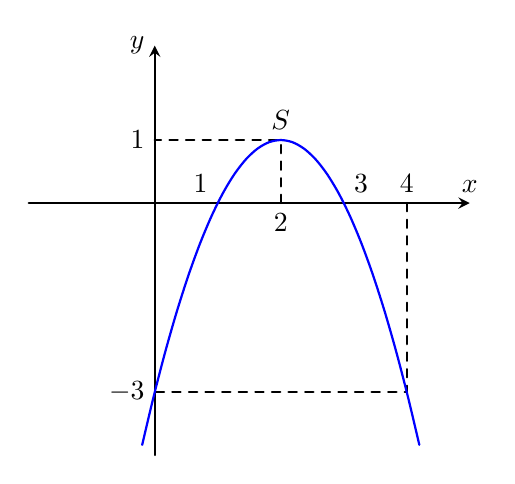
\begin{tikzpicture}[scale=0.8,line cap=round, line join=round, >=stealth, thick]
					\def\xmin{-2}
					\def\xmax{5}
					\def\ymin{-4}
					\def\ymax{2.5}
					\path
					(0,-3) coordinate (A)node[left]{$-3$}
					(1,0) coordinate (B)node[above left]{$1$}
					(2,1) coordinate (C)node[above]{$S$}
					(3,0) coordinate (D)node[above right]{$3$}
					(4,-3) coordinate (E)
					;
					\draw[-stealth] (\xmin,0)--(\xmax,0)node[above]{$x$};
					\draw[-stealth] (0,\ymin)--(0,\ymax)node[left]{$y$};
					\draw[dashed] (2,0)node[below]{$2$}--(2,1)--(0,1)node[left]{$1$} (4,0)node[above]{$4$}--(4,-3)--(0,-3);
					\draw[blue, domain = \xmin+1.8:\xmax-0.8,smooth=200]plot(\x,{-(\x)^2+4*(\x)-3});
				\end{tikzpicture}
			\end{center}
		\end{enumerate}
	}
\end{bt}


\begin{bt}%[0T4B3-1]%[Dự án đề kiểm tra HK1 NH22-23]%[Tạ Quang Bửu]%Lê Hùng Thắng
\immini [thm]{Các nhà khảo cổ học tìm được một mảnh chiếc đĩa cổ hình tròn bị vỡ. Để xác định bán kính của chiếc đĩa, các nhà khảo cổ lấy 3 điểm trên vành đĩa và tiến hành đo đạc thu được kết quả như sau
$BC=28$ cm; $\widehat{BAC}=120^{\circ}$ (Hình vẽ). Tính bán kính của chiếc đĩa (làm tròn kết quả đển hàng phần nghìn).
}
{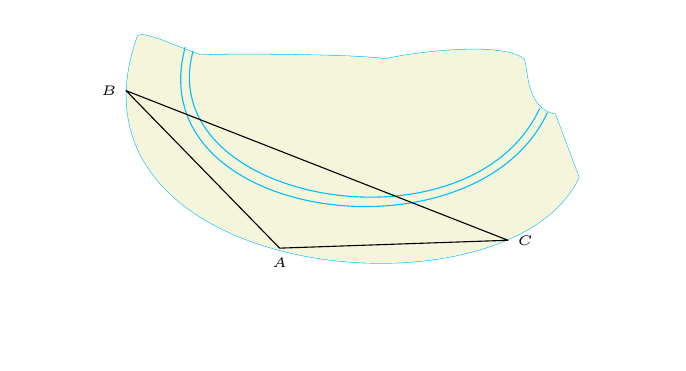
\begin{tikzpicture}[line join=round, line cap=round,scale=1,transform shape]
	\definecolor{beige}{rgb}{0.96, 0.96, 0.86}
	\definecolor{deepskyblue}{rgb}{0.0, 0.75, 1.0}
	\clip (-4,-2.5) rectangle (4,1.5);
	\tikzset{chen/.pic={
	\def\C{ %sóng
	(-2.6,1.4)
	..controls +(-110:3.32) and +(-115:2.1) ..(3,-.4)--(2.7,.4)
	..controls +(170:.4) and +(-55:.1) ..(2.3,1.1)
	..controls +(140:.4) and +(25:.1) ..(.55,1.1)
	..controls +(170:.4) and +(10:.1) ..(-1.8,1.15)
	..controls +(160:.4) and +(30:.1) ..(-2.6,1.4)
	;}
	\draw[color=deepskyblue] \C;
	\fill[beige] \C;
	\def\c{ %sóng
	(-1.9,1.2) ..controls +(-105:2) and +(-115:2.1) ..(2.5,.47)
	(-2,1.25) ..controls +(-105:2.3) and +(-115:2.15) ..(2.6,.42)	;}
	\draw[color=deepskyblue] \c;
	}}
	\path	(0,0)pic[scale=1]{chen}	;
	\path 	(-.8,-1.3) coordinate (A)
	(-2.75,.7) coordinate (B)
	(2.1,-1.2) coordinate (C)	;
	\node at (B) [left]{\tiny $B$};
	\node at (A) [below]{\tiny $A$};
	\node at (C) [right]{\tiny $C$};
	\draw (B)--(C)--(A)--cycle;
	\end{tikzpicture}
}

	\dapso{$16{,}166$ cm }
	\loigiai{Gọi $R$ là bán kính của cái đĩa. Ta có $R$ là bán kính đường tròn ngoại tiếp $\triangle ABC$ suy ra\\
	$\dfrac{BC}{\sin \widehat{BAC}}=2R \Leftrightarrow R= \dfrac{BC}{2 \sin A}  \Leftrightarrow R= \dfrac{28}{2 \sin 120^\circ} \approx 16{,}166$. 
	}
\end{bt} 

\begin{bt}%[0T4B3-1]%[Dự án đề kiểm tra HK1 NH22-23]%[Tạ Quang Bửu]%Lê Hùng Thắng
Tính diện tích một lá cờ hình tam giác cân. Biết lá cờ đó có chiều dài cạnh bên là $32$ cm và góc ở đáy có số đo là $48^{\circ}$ (làm tròn kết quả đến hàng phần nghìn).
\dapso{$509{,}195$ cm$^2$ }
\loigiai{
\immini{
Xét lá cờ có dạng tam giác cân $ABC$. Gọi $H$ là trung điểm của $BC$.\\
Ta có $\cos \widehat{HCA} = \dfrac{HC}{AC} \Rightarrow HC =AC \cdot \cos 48^\circ$.\\
Diện tích tam giác $ABC$ là\\
\allowdisplaybreaks
$\begin{aligned}[t]
	S_{\triangle ABC}=2 S_{\triangle AHC} & = CH \cdot CA \sin 48^\circ \\
	 & =AC \cdot \cos 48^\circ \cdot CA \sin 48^\circ \approx 509{,}195 \mathrm{cm}^2.
\end{aligned}
$
}
{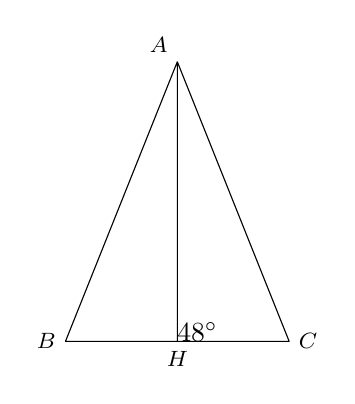
\begin{tikzpicture}[scale=0.71,>=stealth, font=\footnotesize, line join=round, line cap=round]
\path (0,0) coordinate (H)
(0,5) coordinate (A)
(-2,0) coordinate (B)
(2,0) coordinate (C);
\draw (H) node [below] {$H$}-
-(A) node [above left] {$A$}--(B) node [left] {$B$}--(C) node [right] {$C$}--(A);
%\tkzMarkAngles[size=0.7cm](A,C,B)
\tkzMarkAngles[size=0.5cm,arc=l,mark=](A,C,B)
\tkzLabelAngles[pos=0.91,rotate=60](A,C,B){$48^\circ$}
\tkzMarkRightAngles[size=0.25](C,H,A)
\end{tikzpicture}
}
}
\end{bt} 

\begin{bt}%[0T5K3-4]%[Dự án đề kiểm tra HK1 NH22-23]%[Tạ Quang Bửu]%Lê Hùng Thắng
	Cho tam giác $A B C$ có trung tuyến $A M$. Gọi $I$ là trung điểm của $A M$ và $K$ là điểm trên cạnh $A C$ sao cho $A K=\dfrac{1}{3} A C$.
	\begin{enumerate}
	\item Chứng minh $\vec{B I}=\dfrac{1}{2} \vec{B A}+\dfrac{1}{4} \vec{B C}$.
	\item Tính $\vec{B K}$ theo $\vec{B A}, \vec{B C}$.
	\item Chứng minh ba điểm $B,~ I,~ K$ thẳng hàng.
	\end{enumerate}
	\dapso{a) $\vec{B I}=\dfrac{1}{2} \vec{B A}+\dfrac{1}{4} \vec{B C}$ ; b) $\vec{B K}=\dfrac{2}{3}\vec{BA}+\dfrac{1}{3}\vec{B C}$ ; c) Ba điểm $B,~ I,~ K$ thẳng hàng. }
	\loigiai{
	\begin{enumerate}
\immini{
	\item Vì $I$ là trung điểm của $AM$ nên ta có\\
	\allowdisplaybreaks
	$\begin{aligned}[t]
	 2\vec {BI} & = \vec{BA} +\vec{BM} \\
	\Rightarrow \vec{BI} & = \dfrac{1}{2}\vec{BA} +\dfrac{1}{2} \vec{BM}\\ 
	& = \dfrac{1}{2} \vec{BA}+\dfrac{1}{4} \vec{BC}.
	\end{aligned}$

}	
{\begin{tikzpicture}[scale=0.71,>=stealth, font=\footnotesize, line join=round, line cap=round]
	\path (0,4) coordinate (A)
	(-2,0) coordinate (B)
	(4,0) coordinate (C)
	($(B)!0.5!(C)$) coordinate (M)
	($(A)!0.5!(M)$) coordinate (I)
	($(A)!1/3!(C)$) coordinate (K);
	\draw (A)--(B)--(C)--(A)--(M) (B)--(K);
\foreach \d/\g in {A/150,B/180,C/0,M/-90,I/180,K/30} \fill (\d) circle (1pt) ++(\g: 3mm) node {$\d$};
\end{tikzpicture}
}
	\item Ta có \allowdisplaybreaks
	$\begin{aligned}[t]
	\vec {BK} & = \vec{BA} +\vec{AK} \\
	 & = \vec{BA} +\dfrac{1}{3} \vec{AC}\\ 
	& = \vec{BA}+\dfrac{1}{3}(\vec{BC}- \vec{BA})\\
	& = \dfrac{2}{3}\vec{BA}+\dfrac{1}{3} \vec{BC}.
	\end{aligned}$
	\item Ta có 
	$\vec {BI} =\dfrac{1}{2}\vec{BA}+\dfrac{1}{4} \vec{BC}$ và	$\vec {BK} =\dfrac{2}{3}\vec{BA}+\dfrac{1}{3} \vec{BC}$.\\
	Suy ra $\vec{B I} =\dfrac{3}{4} \vec{B K}$.\\
	Vậy ba điểm $B,~ I,~ K$ thẳng hàng.
\end{enumerate}
	}
\end{bt}
\begin{bt}%[0T5B4-1]%[Dự án đề kiểm tra HK1 NH22-23]%[Tạ Quang Bửu]%Lê Hùng Thắng
	Cho tam giác đều $A B C$ có cạnh bằng $2$ và có đường cao $A H$. Tính các tích vô hướng.
	\begin{listEX}[2]
	\item $\vec{A B} \cdot \vec{A C}$.
	\item $\vec{A H}\cdot \vec{B C}$.
	\end{listEX}
	\dapso{ a) $\vec{A B} \cdot \vec{A C}=2$ ; b) $\vec{A H}\cdot \vec{B C}=0$}
	\loigiai{
	\immini{
	\begin{enumerate}
	\item \allowdisplaybreaks
	$\begin{aligned}[t]
	\vec{A B} \cdot \vec{A C} & = AB\cdot AC \cdot \cos (\vec{A B},\vec{A C}) \\
	& = 2\cdot 2 \cdot \cos 60^\circ = 2.
	\end{aligned}$	
	\item \allowdisplaybreaks
	$\begin{aligned}[t]
	\vec{AH} \cdot \vec{BC} & = AH\cdot BC \cdot \cos (\vec{A H},\vec{BC}) \\
	& = AH \cdot BC \cdot \cos 90^\circ = 0.
	\end{aligned}$	
	\end{enumerate}
}
	{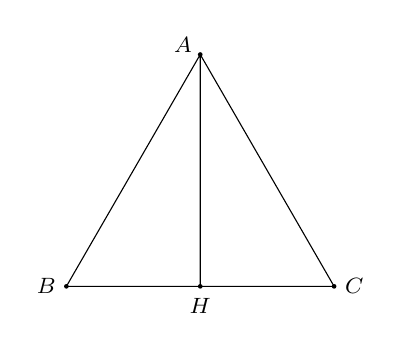
\begin{tikzpicture}[scale=0.85,>=stealth, font=\footnotesize, line join=round, line cap=round]
	\path (-2,0) coordinate (B)
	(2,0) coordinate (C)
	(0,0) coordinate (H);
	\draw (B)--(C)--([turn]120:4) coordinate(A)--cycle (A)--(H);%
	\foreach \d/\g in {A/150,B/180,C/0,H/-90} \fill (\d) circle (1pt) ++(\g: 3mm) node {$\d$};
	\tkzMarkRightAngles[size=0.2](C,H,A)
	\end{tikzpicture}	

}
	}
\end{bt}


